% !TEX program = lualatex
%==============================================================================
% プリアンブル (Preamble)
%==============================================================================

% ===== ドキュメントクラス =====
\documentclass[
    a4paper,
    11pt
]{ltjsreport}

%------------------------------------------------------------------------------
% パッケージ読み込み
%------------------------------------------------------------------------------

% ===== フォント・言語設定 (LuaLaTeX専用) =====
\usepackage{luatexja-fontspec}
\usepackage{lmodern} % フォントサイズの置き換えを防ぐため

% ===== レイアウト関連 =====
\usepackage[margin=2.5cm]{geometry}
\usepackage{booktabs}
\usepackage{float}
\usepackage{graphicx}

% ===== 数式・物理単位関連 =====
\usepackage{amsmath}
\usepackage{siunitx}
\usepackage{bm} % ベクトルを太字にするため (\bm)

% ===== その他 =====
\usepackage{url} % URLを適切に表示
\usepackage{xurl} % Improved line breaking for long URLs
\urlstyle{same}
\Urlmuskip=0mu plus 2mu
\usepackage[
  hidelinks,
]{hyperref}

%------------------------------------------------------------------------------
% 各種設定
%------------------------------------------------------------------------------

% ===== フォント設定 =====
\setmainfont{Latin Modern Roman}
\setsansfont{Latin Modern Sans}
\setmonofont{Latin Modern Mono}
\setmainjfont[Renderer=HarfBuzz]{Yu Mincho}
\setsansjfont[Renderer=HarfBuzz]{Yu Gothic}
\DeclareMathSizes{11}{11}{7}{5} % 数学フォントサイズの調整

% ===== ドキュメント情報 =====
\title{高周波基板における伝送損失の物理的起源と\\高精度分離測定に関する体系的研究}
\author{(氏名)}
\date{\today}

% ===== 数式用カスタムコマンド =====
\providecommand{\dd}{\mathrm{d}} % 微分演算子 d
\newcommand{\mi}{\mathrm{j}} % 虚数単位 j

%==============================================================================
% ドキュメント本体 (Body)
%==============================================================================
\begin{document}
\sloppy % allow more flexible spacing to reduce overfull \hbox warnings

\maketitle
\tableofcontents
\clearpage

% ===================================================================
\chapter*{序論:研究の核心的課題 — 「損失の分離」と「実効的導電率」}
\addcontentsline{toc}{chapter}{序論:研究の核心的課題 — 「損失の分離」と「実効的導電率」}
% ===================================================================

柳原さん,あなたの研究発表資料\cite{Yanagihara2025}を拝見しました.「BCDRを用いた基板の誘電損失と表面粗さによる電気伝導性の測定」という研究テーマは,\SI{100}{\giga\hertz}級の通信\cite{Yanagihara2025}を支える高周波工学において,最も本質的かつ重要な課題の一つである「損失の分離(Loss Separation)」に正面から取り組むものです.

この課題は,現代の回路設計に不可欠な電磁界シミュレーション技術とも密接に関連しています.高周波回路設計で多用されるFDTD法などのシミュレーションでは,計算コストの制約から導体を損失ゼロの「完全導体(Perfect Electric Conductor, PEC)」として扱うことが多く,これでは現実の導体損失を評価できません.より高精度な解析のために導体に有限の導電率を与えようとしても,高周波領域では「表皮効果」と「表面粗さ」の影響で,銅の物性値(バルク導電率)と実際の振る舞いが大きく乖離します.このシミュレーションと現実のギャップを埋める鍵が,現実の物理効果をすべて含んだ\textbf{「実効的導電率」}を実験的に求めることです.

あなたの研究の最終目的は,この実効的導電率を決定するために不可欠な,導体損失 $\alpha_c$(あるいは $Q_c$)に対する「表面粗さ」の影響を明らかにすることです\cite{Yanagihara2025}.しかし,VNA(ベクトルネットワークアナライザ)で測定できるのは,常に「全体の損失」でしかありません.
\begin{align}
  \alpha &= \alpha_c + \alpha_d \\
  \frac{1}{Q} &= \frac{1}{Q_c} + \frac{1}{Q_d}
\end{align}
したがって,あなたの研究の論理構造は,必然的に以下の2段階測定アプローチとなります.
\begin{enumerate}
  \item \textbf{目的:} 表面粗さの影響を含む真の導体損失 $\alpha_c$(実効的導電率)を知りたい.
  \item \textbf{課題:} しかし測定できるのは全体の損失だけであり,$\alpha_c$ と $\alpha_d$ は共に未知数である.
  \item \textbf{解決策(2段階アプローチ):}
    \begin{description}
        \item[Step 1: 基準測定] 評価対象の基板から銅箔を完全に除去した「誘電体コア材」を,鏡面仕上げの基準電極で測定する.これにより,材料固有の純粋な誘電損失 $\alpha_d$(すなわち $\tan\delta$ や $Q_d$)を精密に決定する.
        \item[Step 2: 本測定] 次に,表面粗さを持つ銅箔付きの「評価試料」を測定し,全体の損失を求める.その全体の損失から,Step 1で得た既知の誘電損失 $\alpha_d$ を差し引くことで,目的である導体損失 $\alpha_c$ を正確に分離する.
    \end{description}
\end{enumerate}

\clearpage
% ===================================================================
\part{損失の物理的起源と理論的定式化}
% ===================================================================

% ===================================================================
\chapter{誘電損失のミクロな機構}
% ===================================================================
誘電損失は,基板の絶縁体部分(FR-4やMEGTRON6の樹脂やガラスクロス)で発生する熱損失です.その根源は,物質を構成する分子レベルの「分極の遅れ」にあります\cite{wiki:dielectric}.

\section{分極の「遅れ」と熱発生のメカニズム}
\begin{enumerate}
  \item \textbf{分極とは:} 誘電体(絶縁体)に外部から電界 $\bm{E}$ を印加すると,物質内のプラスとマイナスの電荷がわずかに変位し,物質内部に外部電界を打ち消す方向の電界が生じます.この現象を「分極(Polarization)」と呼びます.
  \item \textbf{分極の種類:} 分極には,電子分極,イオン分極,そして水(H\textsubscript{2}O)のように元々極性を持つ分子(双極子)が電界の向きに配向しようとする「双極子配向分極」などがあります\cite{ACSPublications:2014}.
  \item \textbf{高周波における「遅れ」:} あなたが扱うFR-4やMEGTRON6のような高分子材料では,この双極子配向分極がギガヘルツ帯の損失の主要因となります.周波数が高くなると,電界の振動があまりにも速くなるため,分子はそれ自体の質量(慣性)や,周囲の分子との「粘性抵抗」(摩擦)があるため,電界の変化に完全には追従できなくなります\cite{wiki:dielectric}.これが「分極の遅れ」です.
  \item \textbf{熱発生のメカニズム:} この「遅れ」こそが損失の正体です.外部電界は分子を無理やり振動させようとし,分子は粘性抵抗に逆らいながら追従しようとします.この過程で,外部電界が分子群に行った仕事が,分子のランダムな運動(熱)として散逸します\cite{wiki:dielectric}.
\end{enumerate}

\section{\texorpdfstring{複素誘電率($\epsilon = \epsilon' - \mi\epsilon''$)の物理的意味}{複素誘電率の物理的意味}}
この「分極の遅れ」という物理現象を,電磁気学の数式で表現する道具が「複素誘電率」です.電界 $E$ と物質の応答である電束密度 $D$ の間に位相の遅れ $\delta$ が生じる($D(t) \propto \cos(\omega t - \delta)$)ことを表現するため,誘電率 $\epsilon$ は必然的に複素数 $\epsilon = \epsilon' - \mi\epsilon''$ となります.

\begin{itemize}
    \item \textbf{実数部 $\epsilon'$(イプシロン・プライム):} 電界 $E$ と\textbf{同位相}の応答成分を表し,電界エネルギーを物質内部に\textbf{「蓄積」}する能力の大きさを示します\cite{wiki:permittivity}.これが通常「比誘電率 $\epsilon_r$」と呼ばれるものです($\epsilon' = \epsilon_r \epsilon_0$).
    \item \textbf{虚数部 $\epsilon''$(イプシロン・ダブルプライム):} 電界 $E$ から\textbf{90°遅れた}応答成分を表し,分極の遅れによってエネルギーが熱として\textbf{「損失」}される能力の大きさを示します\cite{Microwaves101:permittivity}.
\end{itemize}

\section{\texorpdfstring{誘電正接($\tan\delta$)の物理的意味}{誘電正接の物理的意味}}
誘電正接(Loss Tangent)は,これら2つの物理量の比として定義されます.
\begin{equation}
  \tan\delta = \frac{\epsilon''}{\epsilon'}
\end{equation}
これは,「1サイクルの間に蓄積されるエネルギー($\epsilon'$)のうち,どれだけの割合が熱として失われるか($\epsilon''$)」を示す,規格化された無次元の損失指標です\cite{Altium:2025}.また,理想的なコンデンサ(電流と電圧の位相差が90°)からの「ズレの角度 $\delta$」の正接(タンジェント)としても解釈できます\cite{HVI:2019}.

% ===================================================================
\chapter{導体損失のミクロな機構}
% ===================================================================
導体損失は,基板の銅配線で発生する抵抗損失(ジュール熱)です.高周波では「表皮効果」と「表面粗さ」が支配的になります.

\section{高周波電流と表皮効果}
表皮効果とは,周波数が高くなるほど,電流が導体の中心部を避けて\textbf{表面に集中して流れる}現象です\cite{MDPI:2023}.これは,導体内部を流れる電流が作る時間変化磁界が,ファラデーの電磁誘導の法則により,導体中心部の電流を妨げる向きの渦電流を誘導するために起こります.

\section{\texorpdfstring{表皮深さ($\delta_s$)を決定する物理パラメータ}{表皮深さを決定する物理パラメータ}}
表皮深さ($\delta_s$)は,電流密度が導体表面の $1/e$(約37\%)にまで減衰する深さであり,以下の式で与えられます\cite{InComplianceMagazine:2025}.
\begin{equation}
    \delta_s = \frac{1}{\sqrt{\pi f \mu \sigma}}
\end{equation}
ここで,$f$ は周波数,$\mu$ は透磁率,$\sigma$ は導電率です.周波数が高いほど,また導電率が高いほど,電流はより薄い表面に集中します.

\section{導体表面粗さと損失増大のメカニズム}
ギガヘルツ帯になると,表皮深さ $\delta_s$ は銅箔の表面粗さ($R_z$ が数\si{\micro\meter}オーダー)と同等か,それよりも浅くなります\cite{ElectronicsOrg:2020}.このとき,主に2つのメカニズムによって損失が増大します.
\begin{enumerate}
    \item \textbf{経路長増大:} 電流は粗さの地形に沿って流れるため,実効的な経路長が長くなり,抵抗値が増大します\cite{PolarInstruments:2025}.
    \item \textbf{磁界集中:} 粗さの「谷」の部分では電流が集中し,局所的に磁界が強まります.この強まった磁界が,さらに強力な渦電流(損失)を誘導します.
\end{enumerate}

% ===================================================================
\chapter{伝送線路における損失の数学的表現}
% ===================================================================

\section{伝送線路方程式(電信方程式)からの出発}
伝送線路上の電圧 $V(z)$ と電流 $I(z)$ の振る舞いは,以下の電信方程式で記述されます.
\begin{align}
    -\frac{\dd V(z)}{\dd z} &= (R + \mi\omega L) I(z) \\
    -\frac{\dd I(z)}{\dd z} &= (G + \mi\omega C) V(z)
\end{align}
ここで,$R, L, G, C$ は線路の単位長さあたりの分布定数です.

\section{\texorpdfstring{伝搬定数($\gamma$)の厳密な導出}{伝搬定数の厳密な導出}}
電信方程式から波動方程式を導くと,複素伝搬定数 $\gamma = \alpha + \mi\beta$ が以下のように定義されます.
\begin{equation}
    \gamma^2 = (R + \mi\omega L)(G + \mi\omega C)
\end{equation}
$\gamma$ の実数部である減衰定数 $\alpha$ の厳密な一般式は以下となります.
\begin{equation}
    \alpha = \sqrt{\frac{1}{2} \left\{ \sqrt{(R^2+\omega^2L^2)(G^2+\omega^2C^2)} + (RG - \omega^2 LC) \right\}}
\end{equation}

\section{\texorpdfstring{低損失近似による減衰定数($\alpha$)の導出と損失分離}{低損失近似による減衰定数の導出と損失分離}}
「低損失条件」($R \ll \omega L, G \ll \omega C$)を適用すると,$\alpha$ は以下のように近似できます.
\begin{equation}
    \alpha \approx \frac{R}{2 Z_0} + \frac{G Z_0}{2}
\end{equation}
ここで,$Z_0 \approx \sqrt{L/C}$ は特性インピーダンスです.この式は,全体の減衰 $\alpha$ が,導体損失 $\alpha_c$ と誘電損失 $\alpha_d$ の単純な和で表せることを示しています.
\begin{align}
    \alpha_c &\equiv \frac{R}{2 Z_0} \\
    \alpha_d &\equiv \frac{G Z_0}{2}
\end{align}

\section{\texorpdfstring{各損失成分の周波数特性($\alpha_c \propto \sqrt{f}$, $\alpha_d \propto f$)の導出}{各損失成分の周波数特性の導出}}
\begin{itemize}
    \item \textbf{導体損失 $\alpha_c$:} 高周波抵抗 $R$ は表皮効果により $R \propto \sqrt{f}$ となるため,$\alpha_c \propto \sqrt{f}$ となります.
    \item \textbf{誘電損失 $\alpha_d$:} コンダクタンス $G$ は $G = \omega C \tan\delta \propto f$ となるため,$\alpha_d \propto f$ となります.
\end{itemize}
この周波数依存性の違いが,高周波帯で誘電損失が支配的になる物理的な理由です.

\clearpage
% ===================================================================
\part{高精度測定の原理と実践}
% ===================================================================

% ===================================================================
\chapter{高周波測定の基礎:SパラメータとVNA}
% ===================================================================

\section{なぜSパラメータが必要か}
マイクロ波・ミリ波領域では,理想的な短絡・開放が作れず,プローブの接触自体が回路特性を乱すため,電圧・電流の直接測定は困難です.そのため,電力の流れを「波」として捉え,その散乱(Scattering)の様子を記述するSパラメータが用いられます.

\section{Sパラメータの物理的定義}
Sパラメータは,被測定物(DUT)の各ポートにおける入射波 $a_n$(入力)と出射波 $b_n$(応答)の関係を行列で記述します.2ポートネットワークの場合,
\begin{equation}
    \begin{pmatrix} b_1 \\ b_2 \end{pmatrix}
    =
    \begin{pmatrix} S_{11} & S_{12} \\ S_{21} & S_{22} \end{pmatrix}
    \begin{pmatrix} a_1 \\ a_2 \end{pmatrix}
\end{equation}
各要素は,$S_{11}$ が入力反射係数,$S_{21}$ が順方向透過係数を表し,振幅と位相を持つ複素数です.

\section{VNAによる複素Sパラメータの測定原理}
VNA(ベクトルネットワークアナライザ)は,Sパラメータのベクトル量(振幅と位相)を測定する装置です.その基本原理は「ヘテロダイン検波」に基づいています\cite{AllAboutCircuits:VNA}.
VNAは,DUTへの入力波(基準波)とDUTからの出力波(測定波)をそれぞれ捕捉し,内部の局部発振器(LO)からの信号と混合(Mix)します.これにより,元のギガヘルツ信号が持つ振幅比と位相差の情報を保持したまま,扱いやすい低い中間周波数(IF)に変換します.VNAのDSPは,このIF信号を比較することで,振幅 $|S_{21}|$ と位相 $\angle S_{21}$ を高精度に算出します.

% ===================================================================
\chapter{共振器法による損失の増幅}
% ===================================================================

\section{「共振」の物理的状態:定在波の形成とエネルギーの蓄積}
共振とは,共振器構造に入射した波が反射波と位相が一致して強め合い(建設的干渉),空間的に振幅が固定された「定在波」を形成する状態です\cite{Warwick:resonator}.このとき,共振器内部には外部の何倍もの強大な電磁界エネルギーが蓄積されます\cite{MIT:ResonantCavities}.

\section{Q値(Quality Factor)の多角的理解}
Q値は,共振器が「どれだけ上手に(損失を少なく)エネルギーを蓄積できるか」を示す指標で,3つの等価な側面から理解できます.
\begin{enumerate}
    \item \textbf{エネルギー定義:} $Q = \omega_r (W_{\mathrm{stored}} / P_{\mathrm{loss}})$.蓄積エネルギーと消費電力の比で,最も根本的な定義です\cite{TaylorFrancis:Qfactor}.
    \item \textbf{周波数応答:} $Q_L = f_r / \Delta f_{\mathrm{3dB}}$.共振ピークの鋭さを表し,VNAで直接観測する量です.Q値が高い(低損失)ほどピークは鋭くなります\cite{wiki:Qfactor}.
    \item \textbf{時間応答:} エネルギー供給を止めた後の減衰の遅さを表します.Q値が高いほど,エネルギーはゆっくりと減衰します(鐘の余韻が長い)\cite{wiki:Qfactor}.
\end{enumerate}

\section{共振器法が低損失材料測定に優れる本質的理由}
MEGTRON6のような超低損失材料では,伝送線路法(TL法)で測定する減衰量 $\alpha$ が小さすぎて測定誤差に埋もれてしまいます.
共振器法は,時間的にエネルギーを蓄積すること(Q回往復させること)で,材料の微小な損失($\tan\delta$)を,VNAで高精度に測定可能な「周波数幅($\Delta f$)」という指標に高感度に変換します.これは,微小な損失の影響を「増幅」して観測する手法と言え,低損失材料の精密測定に不可欠です.

% ===================================================================
\chapter{BCDR法の原理と実践}
% ===================================================================

\section{\texorpdfstring{BCDRが利用するTM\textsubscript{0m0}モードの電磁界分布とその役割}{BCDRが利用するTM0m0モードの電磁界分布とその役割}}
BCDR(Balanced Circular Disk Resonator)法では,円筒対称な TM\textsubscript{0m0} モードを選択的に利用します\cite{IEEE:BCDR220GHz}.このモードは,電界 $E$ が基板に垂直な $z$ 成分のみ,磁界 $H$ が同心円状の $\phi$ 成分のみを持つという非常にシンプルな電磁界分布をしています\cite{ScholarsMine:TM010}.基板の厚さ方向の誘電特性($\epsilon_r, \tan\delta$)を測定するのに最も適したモードです.

\section{S21共振ピークからの物性値算出プロセス(一般論)}
VNAで測定したS21の生データから物性値を導出する一般的なプロセスは,以下の通りです.
\begin{enumerate}
    \item \textbf{負荷Q($Q_L$)の測定:} VNAのマーカー機能で共振周波数 $f_r$ と半値全幅 $\Delta f$ を読み取り,$Q_L = f_r / \Delta f$ を算出します.
    \item \textbf{無負荷Q($Q_0$)の算出:} 負荷Q $Q_L$ とピークの挿入損失 $IL_r$ から,測定系との結合による外部損失を取り除いた,共振器自体の真のQ値である無負荷Q $Q_0$ を算出します:$Q_0 = Q_L / (1 - 10^{IL_r / 20})$.
    \item \textbf{比誘電率 $\epsilon_r$ の算出:} 測定した共振周波数 $f_r$ とBCDRの寸法から,理論式(超越方程式)を数値的に解くことで $\epsilon_r$ を決定します.
    \item \textbf{損失の分離計算:} 全体の損失を表す $1/Q_0$ は,導体損失 $1/Q_c$ と誘電損失 $1/Q_d$ の和($1/Q_0 = 1/Q_c + 1/Q_d$)で表されます.$Q_c$ を理論計算し,$Q_0$ から差し引くことで $Q_d$ を分離し,$\tan\delta = 1/Q_d$ を得ます.
\end{enumerate}
しかし,この一般論では導体損失 $Q_c$ の理論計算に「表面粗さ」という不確定要素が含まれるため,高精度な分離は困難です.次章でその解決策を述べます.

% ===================================================================
\chapter{基準測定を用いた高精度損失分離法}
% ===================================================================
単一の測定から誘電損失と表面粗さの影響を分離することは原理的に困難です.この問題を解決するため,「基準測定」と「本測定」を組み合わせた2段階の測定アプローチが極めて有効です.

\section{Step 1: 基準測定による誘電体特性の精密決定}
まず,導体の表面粗さという不確定要素を完全に排除し,誘電体材料固有の損失特性 $\tan\delta$ を正確に決定します.
\begin{enumerate}
    \item \textbf{試料準備:} 評価対象の基板から,化学処理(エッチング)により銅箔を完全に除去した\textbf{誘電体コア材}を用意します.
    \item \textbf{測定:} この誘電体コア材を,表面が極めて平滑な\textbf{標準銅箔(基準電極)}で挟み,BCDR測定を行います.
    \item \textbf{計算:} この系で測定した全体のQ値 $Q_{0,\mathrm{ref}}$ から,表面粗さの影響を無視して理論計算できる基準電極の導体Q値 $Q_{c,\mathrm{ref}}$ を差し引きます.
\end{enumerate}
\begin{equation}
    \tan\delta = \frac{1}{Q_d} = \frac{1}{Q_{0,\mathrm{ref}}} - \frac{1}{Q_{c,\mathrm{ref}}}
\end{equation}
このステップにより,導体損失の不確かさから完全に分離された,信頼性の高い $\tan\delta$ の周波数特性データが得られます.

\section{Step 2: 本測定による実効的導電率の導出}
次に,前節で決定した既知の $\tan\delta$ を用いて,評価対象である実際の基板の導体損失(表面粗さ効果)を分離し,実効的導電率を導出します.
\begin{enumerate}
    \item \textbf{試料準備:} 評価対象である,\textbf{表面粗さを持つ銅箔が貼られたままの基板(DUT)}を用います.
    \item \textbf{測定:} DUTをBCDRで測定し,全体のQ値 $Q_{0,\mathrm{dut}}$ を得ます.
    \item \textbf{計算:} 損失分離式を $Q_{c,\mathrm{dut}}$ について解き,測定した $Q_{0,\mathrm{dut}}$ とStep 1で得た $Q_d$ を用いて,DUTの銅箔が持つ表面粗さの影響を全て含んだ実測の導体損失 $Q_{c,\mathrm{dut}}$ を算出します.
\end{enumerate}
\begin{equation}
    \frac{1}{Q_{c,\mathrm{dut}}} = \frac{1}{Q_{0,\mathrm{dut}}} - \frac{1}{Q_d} = \frac{1}{Q_{0,\mathrm{dut}}} - \tan\delta
\end{equation}
この実測された導体損失 $Q_{c,\mathrm{dut}}$ から,電磁界理論に基づき最終目的である\textbf{実効的導電率 $\sigma_{\mathrm{eff}}$} を算出します.この値こそが,高精度なFDTDシミュレーションに不可欠なパラメータとなります.

\clearpage
% ===================================================================
\part{応用的考察と研究の深化}
% ===================================================================

% ===================================================================
\chapter{損失の周波数特性と材料選定の重要性}
% ===================================================================
\section{理論と実測の比較:各種基板における損失成分の振る舞い}
第I部で導出した通り,導体損失 $\alpha_c$ は $\sqrt{f}$ に,誘電損失 $\alpha_d$ は $f$ に比例します.図\ref{fig:loss_vs_freq}は,汎用的なFR-4基板と高性能な低損失基板について,この関係を実測データで示したものです.

\begin{figure}[H]
    \centering
    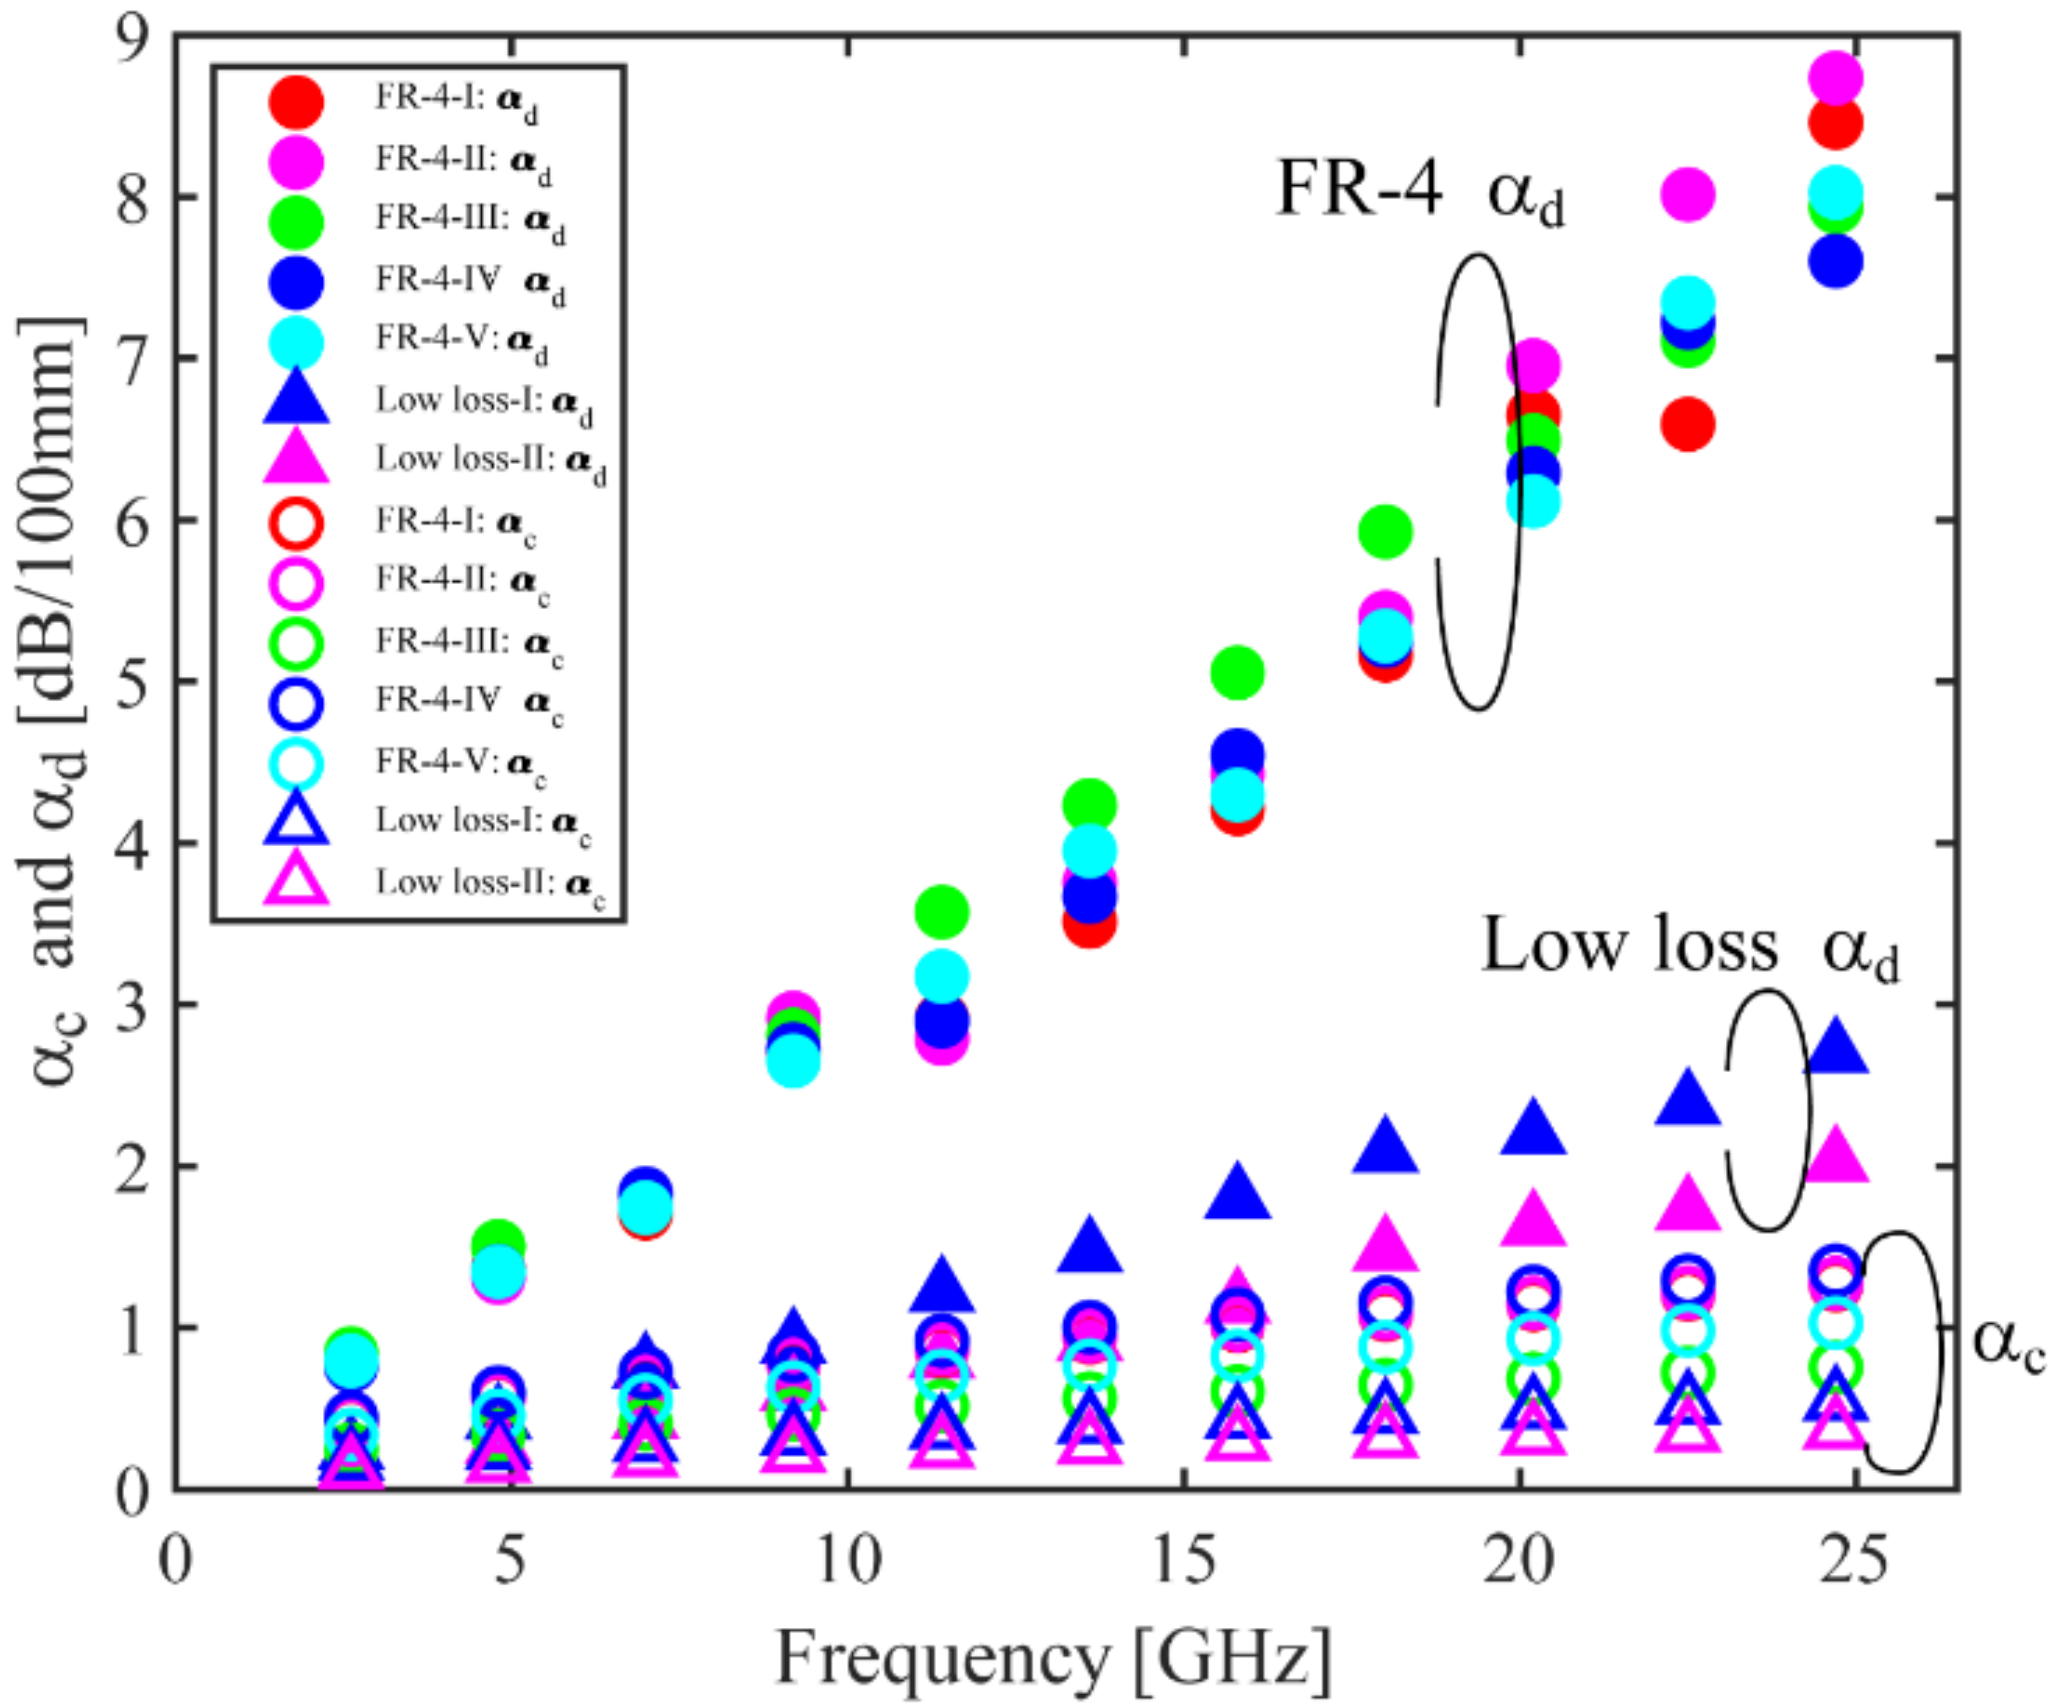
\includegraphics[width=0.8\textwidth]{input_file_0.png}
    \caption{各種基板材料における導体損失($\alpha_c$)と誘電損失($\alpha_d$)の周波数依存性.}
    \label{fig:loss_vs_freq}
\end{figure}

\section{高周波帯で誘電損失が支配的になる物理的理由}
図\ref{fig:loss_vs_freq}が示すように,周波数 $f$ が高くなると,線形に増加する誘電損失 $\alpha_d$ が,緩やかにしか増加しない導体損失 $\alpha_c$ を必ず追い越します.これが,高周波信号伝送において,$\tan\delta$ の小さい低損失材料の選定が極めて重要になる物理的な理由です.

\section{FR-4の利用限界と低損失材料の戦略的価値}
FR-4は低周波域ではコスト面の利点から多用されますが,\SI{20}{\giga\hertz}を超える領域では誘電損失が急激に増大し,信号品質の維持が困難になります.数十Gbpsの高速デジタル伝送やミリ波回路では,$\tan\delta$ の増加勾配が緩やかな低損失材料の採用が,システムの性能を保証する上で不可欠な戦略となります.

% ===================================================================
\chapter{測定精度と不確かさの評価}
% ===================================================================
BCDR法による精密測定といえども,様々な誤差要因が存在します.その影響を理解し,制御することが高精度な評価には不可欠です.

\section{最大の誤差要因:エアギャップの影響}
BCDRの導体板と測定サンプルとの間に生じる,ミクロンレベルのわずかな隙間「エアギャップ」は,最大の誤差要因です\cite{IEEE:BCDR220GHz}.この隙間は,比誘電率が1で損失がゼロの微小なコンデンサがサンプルと直列に接続されたかのような影響を与えます.
これにより,測定される実効的な比誘電率 $\epsilon_r$ は真の値よりも低く,実効的な誘電正接 $\tan\delta$ も,特に低損失材料では真の値より著しく低く見積もられてしまいます.例えば,厚さ\SI{50}{\micro\meter}の基板に対し\SI{5}{\micro\meter}のエアギャップが存在するだけで,$\tan\delta$ が20\%以上も過小評価されるという報告もあります.

\section{高周波域における測定限界:不要モードと放射損失}
高周波になるほど,測定はより困難になります.
\begin{itemize}
    \item \textbf{不要モード(スプリアス)の発生:} 周波数が高くなると,目的のTM\textsubscript{0m0}モード以外に,TEモードやハイブリッドモードといった不要な共振モードが発生しやすくなります.これらが目的のモードと周波数的に近接すると,モードカップリングを起こして共振ピークを歪ませ,Q値の正確な測定を妨げます.
    \item \textbf{放射損失:} 共振器は理想的には閉じた系ですが,実際には側面(開放端)からわずかに電磁波が放射されます.周波数が高くなり波長が短くなると,この放射損失が無視できなくなります.放射損失は導体損失や誘電損失とは別の損失メカニズムであり,これを材料損失と誤認しないよう注意が必要です.
\end{itemize}
これらの影響が顕著になる周波数帯では,測定データを除外するなどの判断が必要となります.

\section{測定系のキャリブレーションと再現性の確保}
VNA自体の精度を保証するためのキャリブレーションはもちろんのこと,BCDR治具の組み立て再現性も重要です.特にエアギャップの量を一定に保つため,サンプルを固定する際の締め付けトルクを管理するなど,測定手順を標準化することが,信頼性の高いデータを取得するための鍵となります.

% ===================================================================
\chapter{超高周波領域における界面効果}
% ===================================================================
ミリ波帯のように表皮深さがサブミクロンオーダーにまで浅くなると,導体の「バルク特性」だけでなく,銅箔と誘電体の「界面」の状態が損失に無視できない影響を及ぼします.

\section{表面粗さモデルの高度化(Hurayモデル等)}
単純な経路長増大モデルでは,特に微細な凹凸構造による損失を正確に表現できません.そこで,より物理的な現実に即したモデルが提案されています.
代表的なものが,雪玉が積み重なった構造を仮定する\textbf{Hurayモデル}です.このモデルは,電流が微小な球体(雪玉)の表面を流れると仮定することで,単純な凹凸だけでなく,半球状の突起が作る局所的な磁界集中効果を考慮に入れることができます.これにより,特にマット面(接着面)の複雑な構造が引き起こす損失増大を,より正確に予測することが可能になります.

\section{銅箔-誘電体界面の化学的影響と実効的導電率}
基板製造プロセスでは,銅箔と樹脂の接着強度を確保するため,銅箔表面に酸化処理(黒化処理)やシランカップリング剤による化学処理が施されます.この数nmから数十nmの薄い「界面層」は,純粋な銅とも誘電体とも異なり,導電率が低く損失の大きい層です.
ミリ波帯では電流がこの界面層を流れる割合が増加するため,銅のバルク導電率から予測されるよりも大きな損失が生じる原因となります.精密な損失モデリングは,この界面層の特性を考慮した「実効的導電率」の概念を導入する必要があります.

\section{今後の課題:界面特性を含めた統合的損失モデルの構築}
今後の超高周波回路設計においては,バルクの誘電特性 ($\epsilon_r, \tan\delta$) と導体特性 ($\sigma$) に加え,表面粗さの物理形状と界面の化学的特性を統合した,より高精度な損失モデルの構築が重要な研究課題となります.

\clearpage
% ===================================================================
\part{総合的理解度と質疑応答への準備}
% ===================================================================

% ===================================================================
\chapter{想定問答集}
% ===================================================================
本研究の理解度を深め,あらゆる角度からの質問に論理的かつ的確に応答できるよう,基礎的な概念から応用的・発展的な内容までを網羅した想定問答集を作成します.

\section{基礎概念に関する問答}
\begin{description}
    \item[Q1.] \textbf{そもそも「損失」とは,物理的に何が起きている現象ですか? なぜ高周波になると,損失が問題になるのでしょうか?}
    \item[A1.] はい.「損失」とは,伝送線路を伝わる電気信号のエネルギーが,意図せず「熱」に変わってしまう現象を指します.
    高周波になると問題になる理由は2つあります.第一に,周波数が高くなるほど,誘電損失(基板の樹脂が原因)や導体損失(銅箔が原因)といった熱に変わるメカニズムがより活発に働くため,損失の絶対量が増加します.第二に,デジタル信号は高速化(高周波化)するほど,信号の波形がなまりやすくなります.損失が大きいと,この波形のなまりが酷くなり,「0」と「1」の区別がつかなくなって通信エラーを引き起こすため,高周波ほど深刻な問題となります.

    \item[Q2.] \textbf{なぜ損失を「導体損失」と「誘電損失」の2つに『分離』して考える必要があるのですか? 全体の損失だけを見ていては,なぜ不十分なのでしょうか?}
    \item[A2.] それは,損失の原因を正確に特定し,適切な対策を打つためです.例えば,ある基板の全体損失が大きい場合,その原因が「銅箔の表面の粗さ」なのか,それとも「基板の樹脂材料の特性」なのかを切り分けなければ,改善のしようがありません.
    導体損失が原因であれば,より表面が平滑な銅箔を採用するべき,という結論になります.一方で,誘電損失が原因であれば,より高性能な低損失材料に変更するべき,となります.このように,原因によって対策が全く異なるため,損失をその物理的な起源ごとに分離して評価することが,材料開発や回路設計において不可欠なのです.

    \item[Q3.] \textbf{「比誘電率 ($\epsilon_r$)」と「誘電正接 ($\tan\delta$)」は,基板の性能指標としてよく聞きますが,この2つは何が違うのですか?}
    \item[A3.] はい.この2つは役割が全く異なります.
    \textbf{比誘電率 ($\epsilon_r$)} は,主に「信号の伝わる速さ」と「回路の物理的なサイズ」を決定します.$\epsilon_r$ が高いほど信号は遅くなります.いわば,信号が伝わる「道の舗装状態」を決めるパラメータです.
    一方,\textbf{誘電正接 ($\tan\delta$)} は,信号が伝わる際の「エネルギー損失の大きさ」を決定します.$\tan\delta$ が大きいほど,信号のエネルギーが熱として失われ,信号が弱まります.これは「道の燃費」に相当するパラメータです.
\end{description}

\section{測定原理に関する問答}
\begin{description}
    \item[Q4.] \textbf{なぜ測定にVNA(ベクトルネットワークアナライザ)を使うのですか? オシロスコープで波形を見るだけでは,損失は分からないのでしょうか?}
    \item[A4.] はい,オシロスコープでは正確な損失測定は困難です.高周波の世界では,信号が単純に弱まるだけでなく,インピーダンスの不整合によって「反射」が起こります.
    VNAは,自身が発生させた基準となる波に対して,被測定物から「どれだけ反射してきたか($S_{11}$)」と「どれだけ透過してきたか($S_{21}$)」を,振幅と位相の両方で極めて精密に測定できる装置です.損失は,この透過してきた波($S_{21}$)がどれだけ減少したかを測定することで評価します.このように,入力波と出力波を比較し,そのベクトル的な比率を測定するというVNAの基本原理が,損失評価には不可欠となります.

    \item[Q5.] \textbf{共振器を使うと,なぜ感度が良くなるのですか? もっと簡単なイメージで教えてください。}
    \item[A5.] はい.これは「ブランコをタイミング良く押し続けると,少しの力でも非常に大きく揺れる」のと同じ原理です.
    共振器は,特定の周波数の電磁波だけを内部に閉じ込めて何千回と往復させ,エネルギーを蓄積します.材料が持つごくわずかな損失は,この「1回の往復」ごとにエネルギーを少しずつ奪っていきますが,何千回も往復させることでその微小な損失が積み重なり,VNAでも観測できるほど大きな変化,すなわち「共振のピークが鈍る」という形で現れます.
    このように,共振器は「時間を利用して損失の影響を増幅する装置」とイメージできます.

    \item[Q6.] \textbf{なぜ単純な伝送線路法(TL法)ではなく,わざわざBCDRのような共振器法を用いるのですか?その本質的な利点は何ですか?}
    \item[A6.] はい.TL法は信号の減衰定数 $\alpha$ を直接測定しますが,今回測定対象としたMEGTRON6\cite{Yanagihara2025}のような超低損失材料では $\alpha$ が極めて小さく,VNAの測定誤差内で有意な減衰を得るには,非現実的な線路長が必要となります.
    共振器法は,電磁界エネルギーをQ値倍に共振器内部に蓄積させ,材料の微小な損失($\tan\delta$)を,「共振ピークの鋭さ($Q=f_r/\Delta f$)」という,VNAで高精度に測定可能な周波数指標に高感度に変換します.この「損失の増幅効果」が,低損失材料の精密測定における共振器法の本質的な利点です.

    \item[Q7.] \textbf{VNAはどのようにしてSパラメータの「位相」を測定しているのですか? ギガヘルツの波の位相を直接測るのは困難ではないですか?}
    \item[A7.] 非常に良いご質問です.VNAはギガヘルツの位相を\textbf{直接}測定しているわけではなく,\textbf{ヘテロダイン検波}という原理を用いています\cite{AllAboutCircuits:VNA}.VNAは,基準信号と測定信号を,内部の局部発振器と混合することで,元のギガヘルツ信号が持つ位相差情報をそのまま保持した,扱いやすい低い\textbf{中間周波数(IF)}の信号に変換します.VNAは,このIF信号間の位相差をデジタル的に精密測定することで,$\angle S_{21}$ を算出しています.
    
    \item[Q8.] \textbf{BCDR法では TM\textsubscript{0m0} モードを利用するとのことですが,このモードが誘電体シートの測定に適しているのはなぜですか?}
    \item[A8.] TM\textsubscript{0m0} モードは,電界 $E$ が基板に対して垂直な成分($E_z$)のみを持ち,磁界 $H$ が同心円状の成分($H_\phi$)のみを持つ,非常にシンプルな円筒対称のモードです\cite{ScholarsMine:TM010}.基板材料の $\epsilon_r$ や $\tan\delta$ は,主に電界によって決まる物性です.$E_z$ が基板全面に一様に印加されるこのモードは,基板の厚さ方向の誘電特性を測定する上で,最も理想的かつ解析しやすい電磁界分布であるため,選択的に利用されます.
\end{description}

\section{物理機構と理論に関する問答}
\begin{description}
    \item[Q9.] \textbf{導体表面の粗さ(Roughness)が損失を増やす物理的メカニズムを,表皮深さ(Skin Depth)と関連付けて説明してください.}
    \item[A9.] はい.高周波では表皮効果により電流が表面の薄い層(表皮深さ $\delta_s$)に集中します.$\delta_s$ が銅箔の表面粗さと同等以下になると,主に2つのメカニズムで損失が増大します.第一に,電流が粗さの凹凸に沿って流れるため,実効的な電流経路長が増大し,抵抗が増加します.第二に,粗さの「谷」部分では,電流が集中し局所的な磁界が強まります.この強まった磁界が,さらに強力な渦電流(損失)を誘導するためです.

    \item[Q10.] \textbf{複素誘電率 $\epsilon = \epsilon' - \mi\epsilon''$ の「虚数部 $\epsilon''$」とは,物理的に何を意味しますか?}
    \item[A10.] 複素誘電率は,物質に印加した電界 $E$ と,それに対する物質の応答(電束密度 $D$)の間の「位相の遅れ」を表現したものです.実数部 $\epsilon'$ は電界と同位相の応答で,エネルギーを「蓄積」する能力($\epsilon_r$)を意味します.虚数部 $\epsilon''$ は電界と90°遅れた応答で,分極が電界に追従しきれないことによる「摩擦」に相当し,1サイクルあたりに熱として「損失」されるエネルギーの大きさを表します.

    \item[Q11.] \textbf{損失の分離式は $1/Q = 1/Q_c + 1/Q_d$ と「逆数の和」で表されます.なぜQそのものの和 $Q = Q_c + Q_d$ ではないのですか?}
    \item[A11.] それは,Q値のエネルギー定義 $Q = \omega W_{\mathrm{stored}} / P_{\mathrm{loss}}$ と,物理法則である「電力の加法性」に基づいています.共振器全体の消費電力 $P_{\mathrm{total}}$ は,導体損失 $P_c$ と誘電損失 $P_d$ の単純な和で表されます.この式の各項をQ値の定義を用いて書き換えると,$1/Q_{\mathrm{total}} = 1/Q_c + 1/Q_d$ という関係が導かれます.つまり,「$1/Q$(損失率)」が,消費電力と同様の加法性を持つためです.

    \item[Q12.] \textbf{減衰定数 $\alpha$ と Q値 の関係式 $\alpha = \beta / (2Q)$ は,どのように導出されるのですか?}
    \item[A12.] はい.この式の厳密な導出は,Qのエネルギー定義から始まります.伝送線路を伝わる電力 $P$ と単位長さあたりの消費電力 $P'_{\mathrm{loss}}$ の間には $P'_{\mathrm{loss}}=2\alpha P$ という関係があります.また,電力 $P$ はエネルギーが伝わる速度,すなわち群速度 $v_g$ で運ばれるため,$P = W'_{\mathrm{stored}} \times v_g$ と表されます.これらを整理すると,厳密な関係式 $\alpha = \omega / (2 Q v_g)$ が得られます.ここで媒質が「無分散」で群速度 $v_g$ と位相速度 $v_p=\omega/\beta$ が等しいと近似できる場合にのみ,ご質問の $\alpha = \beta / (2Q)$ という簡略化された関係式が導出されます.
\end{description}

% ===================================================================
\section{追加の想定問答集}
% ===================================================================
ここでは,発表中によく聞かれる(あるいは核心を突く)追加の質問と,短く簡潔に答えられるサンプル応答をまとめます.単純な単語の意味(定義)も合わせて含めています.

% -----------------------------------
\subsection{単語・用語の短い定義(ワンセンテンス)}
% -----------------------------------
\begin{description}
    \item[表皮効果(Skin effect)] 高周波で電流が導体表面に集中する現象.
    \item[表皮深さ($\delta_s$)] 電流密度が表面の $1/e$ に減衰する深さ.
    \item[比誘電率($\epsilon_r$)] 材料により電界の速度が変化する指標.
    \item[誘電正接($\tan\delta$)] 誘電体の損失度合い(無次元).
    \item[Q値] 共振器がエネルギーを蓄える能力の指標(損失の逆数).
    \item[VNA] Sパラメータの振幅と位相を同時計測する測定器.
    \item[BCDR] 円形共振器を用いた低損失材料評価のための測定法.
    \item[実効的導電率($\sigma_{\mathrm{eff}}$)] 表皮効果・表面粗さ・界面層を含めた実測相当の導電率.
    \item[エアギャップ] 試料と治具の間にある微小な隙間.誘電率測定を低く見積もる主原因.
\end{description}

% -----------------------------------
\subsection{測定法・実験に関するよくある質問}
% -----------------------------------
\begin{description}
    \item[Q.] エアギャップの影響をどう最小化していますか?
    \item[A.] 組み付け時のトルク管理,表面を平滑にするための前処理,薄い導電性ペーストを使用して局所的な接触欠如を補う,複数回測定して一貫性を確認する,など複合的対策をとっています.

    \item[Q.] 表面粗さの代表値は何を使っていますか?$R_a$?$R_z$?
    \item[A.] 測定手法とモデルに依りますが,パワー損失への寄与は高くて局所ピークに敏感なため,$R_z$ や Huray モデルのパラメータ(雪玉半径・密度)を合わせて報告します.

    \item[Q.] 温度変化は結果にどれほど影響しますか?
    \item[A.] 銅の導電率は温度で変化し,$
ho(T)\propto (1+\alpha_T(T-T_0))$ のように線形近似できます.極端な温度変動がある場合は,校正温度での測定か温度補正を行います.実験では室温±1~2\,\si{\celsius} を目安に安定させています.

    \item[Q.] キャリブレーションはどのように行いますか?
    \item[A.] VNAの基本キャリブ(オープン/ショート/ロード/スルー)を実施し,BCDR治具の寄生損失や接続損失は基準測定(標準素材)で補正します.

    \item[Q.] 他の共振器(例えばドーナツ型やストリップライン共振器)との比較は?
    \item[A.] BCDRは円筒対称でTM\textsubscript{0m0}モードが厚み方向の特性を直接反映するため,誘電特性の精密測定に優れます.共振器選択は目的とターゲット周波数に依存しますが,BCDRは薄板評価に適しています.
\end{description}

% -----------------------------------
\subsection{理論・モデリングに関する質問}
% -----------------------------------
\begin{description}
    \item[Q.] Hurayモデルはいつ使うべきですか?単純な経路長モデルではダメなのですか?
    \item[A.] 凹凸のスケールが微小な突起(ナノ〜マイクロ)を含む場合,単純モデルは平均的な経路長増加しか表現できず,局所磁界強度増大を無視します.Hurayモデルはこれを半球体群として扱い,局所的磁界集中を表現できるため精度が向上します.

    \item[Q.] 実効的導電率 $\sigma_{\mathrm{eff}}$ はどのように算出していますか?
    \item[A.] 測定で得た $Q_{c,\mathrm{dut}}$ を電磁界解析(解析解や数値法)で逆算して,導体に与えるべき導電率値(バルクからの減衰を含め)を求めます.表面粗さはモデルで補正します.

    \item[Q.] FDTD等のシミュレーションではPECでなく有限導電率を使うべきか?
    \item[A.] 周波数と目的によりけりですが,100\,\si{\giga\hertz}級では実効的導電率を入れると挙動(損失や位相)が実機により近づきます.PECは計算コストを下げる目的では有用ですが,設計評価には実効値を用いることが望ましいです.
\end{description}

% -----------------------------------
\subsection{データ解析と不確かさに関する質問}
% -----------------------------------
\begin{description}
    \item[Q.] Q値の誤差評価はどのようにしていますか?
    \item[A.] VNAの読み取り精度,ピーク同定の誤差,結合損失の補正誤差,組み付け再現性(エアギャップ)を誤差源として,分散法やモンテカルロ法で $\Delta Q/Q$ を推定します.

    \item[Q.] 周波数依存性はどう扱いますか?単一周波数だけでは不完全では?
    \item[A.] できる限り広帯域で連続した共振周波数を得るか,複数のモード/複数の治具を使って周波数特性を取得します.また,予測モデル($\sqrt{f}$, $f$)とフィッティングして分離の妥当性を評価します.
\end{description}

% -----------------------------------
\subsection{発展的・批判対応の質問}
% -----------------------------------
\begin{description}
    \item[Q.] 結果の一般化はどこまで可能か?別の銅の厚さや被覆処理でも再現できますか?
    \item[A.] 表面粗さ・界面処理・銅厚さは明確に損失に寄与します.本手法は一般化可能ですが,モデルと実測値のマッチングのため,各条件のパラメータ(厚さ・粗さ・処理)を個別に評価し,データベース化する必要があります.

    \item[Q.] 放射損失や不要モードの影響がある周波数帯のデータはどう扱うのか?
    \item[A.] 影響が大きい帯域ではデータを除外するか,別途放射損失項をモデルに追加して補正し,再評価します.また,実験設計段階で不要モードの存在しにくい寸法選定を行います.

    \item[Q.] どのようにしてレビューで厳しい指摘(例えばエアギャップの顕著な影響)に応えるか?
    \item[A.] 事前に感度解析を行い,エアギャップが結果に与える影響の大きさを定量的に示します.また,複数サンプル,複数回測定,異なる治具での再現性データを示して,仮説的な誤差源を否定または補正したデータを提示します.
\end{description}


\section{応用的・実践的な問答}
\begin{description}
    \item[Q13.] \textbf{あなたの研究の最終目的は「表面粗さの影響」を調べることですが,今回の発表では「まず誘電損失を測定」しています.この論理的な繋がりを説明してください.}
    \item[A13.] はい.最終的に知りたいのは導体損失 $Q_c$ ですが,測定できるのは全体の損失 $Q_0$ だけであり,分離式 $1/Q_0 = 1/Q_c + 1/Q_d$ には2つの未知数が含まれます.そこで,まず表面が極めて平滑な「基準系」を用いて,表面粗さの影響を排除した状態で材料固有の真の誘電損失 $Q_d$(すなわち $\tan\delta$)を精密に決定します.次に,その既知となった $Q_d$ を利用して,評価対象である「粗さのある基板」の全体の損失 $Q_0$ から $Q_c$ を正確に分離します.このように,まず $\tan\delta$ を確定させることが,最終目的の論理的な前提となります.

    \item[Q14.] \textbf{あなたのBCDR測定系において,$\epsilon_r$ や $\tan\delta$ の測定精度を左右する,最大の誤差要因は何だと考えますか?}
    \item[A14.] エアギャップ(Air Gap),すなわちBCDRの導体板と測定サンプルとの間に生じる,ミクロンレベルのわずかな隙間だと考えます.このエアギャップは,比誘電率が1のコンデンサが直列に挿入されたかのような影響を与え,測定される実効的な $\epsilon_r$ と $\tan\delta$ を,真の値よりも著しく低く見積もらせる原因となります.

    \item[Q15.] \textbf{BCDR測定において,エアギャップの影響を最小化するために具体的にどのような工夫をすべきですか?また,その影響を補正する数学的な手法は存在しますか?}
    \item[A15.] はい.まず物理的な工夫として,(1)BCDR治具の導体表面を鏡面研磨し平坦度を上げること,(2)サンプル全面に均一な圧力がかかるよう,トルク管理されたネジで締め付けること,が重要です.
    数学的な補正手法も存在します.エアギャップを厚さ $d_g$ の空気層($\epsilon_r=1$)とモデル化し,サンプル(厚さ $d_s$, 比誘電率 $\epsilon_s$)と直列の合成容量として実効誘電率を計算する手法が基本です.さらに高度な手法として,複数の厚さのサンプルを測定し,エアギャップの影響を外挿して取り除く方法や,電磁界シミュレーションを用いてエアギャップの影響を定量評価し,測定値を補正(de-embedding)する方法があります.

    \item[Q16.] \textbf{発表スライドでは,高周波側で共振ピークの形が崩れていますが,これはなぜですか?なぜそのデータを計算から除外したのですか?}
    \item[A16.] ご指摘の通り,高周波領域でピーク形状が崩れています.これは材料特性の劣化ではなく,測定系の限界によるものだと考えています.具体的には,(1)目的のTM\textsubscript{0m0}モード以外の不要なスプリアス共振が発生し干渉を起こしている可能性,(2)周波数が高くなり波長が短くなったことで,共振器の側面からの放射損失が無視できなくなった可能性,が考えられます.これらの不要な損失要因が含まれたデータでは,材料本来の $\tan\delta$ を正確に算出できないため,ピーク形状が理論通り明確な周波数帯のデータのみを使用しました.

    \item[Q17.] \textbf{あなたの研究では導体損失と誘電損失を分離していますが,ミリ波帯では放射損失も無視できない場合があります.BCDR法において,放射損失はどのように抑制あるいは評価できると考えますか?}
    \item[A17.] はい.BCDRは上下を導体で挟んだ「閉鎖型」の共振器であるため,マイクロストリップラインのような「開放型」の構造に比べて,原理的に放射損失が極めて小さいという利点があります.放射は主に共振器の側面(開放端)から起こりますが,特に今回のような高誘電率基板では,電磁界が基板内部によく閉じ込められるため,その影響はさらに抑制されます.
    評価方法としては,直径の異なる複数のBCDRで同一材料を測定し,放射損失の大きさ(寸法に依存)と材料損失(寸法に依存しない)を分離する手法や,電磁界シミュレーションによって放射損失の寄与を理論的に計算し,測定結果から差し引く方法が考えられます.

    \item[Q18.] \textbf{表面粗さの損失への寄与をモデル化する際,単純な経路長増大だけでなく,Hurayモデルのような球体を用いたモデルが提案されているのはなぜですか?その物理的な妥当性は何ですか?}
    \item[A18.] それは,単純な経路長増大(トポロジー効果)だけでは,特に銅箔のマット面(接着面)に見られる複雑な凹凸構造が引き起こす損失を説明しきれないためです.
    Hurayモデルは,粗さの表面を「雪玉(微小な球体)の集合体」としてモデル化します.この物理的な妥当性は,電流が単に凹凸の表面をなぞるだけでなく,半球状の突起の周りに「密集」し,局所的な磁界集中を引き起こすという電磁気的な効果を表現できる点にあります.これにより,単純な経路長モデルでは捉えきれない,近接効果による損失増大をより正確に考慮することができ,特に凹凸が激しい表面の損失を高い精度で予測することが可能になります.
\end{description}

\clearpage
% ===================================================================
\appendix
\part*{付録}
\addcontentsline{toc}{part}{付録}
% ===================================================================

% ===================================================================
\chapter{物理指標の相互関係に関する数学的証明}
% ===================================================================

\section{\texorpdfstring{減衰定数 $\alpha$ と Q値 の関係式 $\alpha = \beta / (2Q)$ の証明}{減衰定数とQ値の関係式の証明}}
この式は,伝送線路における\textbf{空間的減衰}($\alpha$)と,共振器における\textbf{時間的減衰}($Q$)を結びつける重要な関係式です.Q値のエネルギー定義から導出できます.
\begin{enumerate}
    \item \textbf{Q値の定義(単位長さあたり):}
    $Q = \omega \frac{W'_{\mathrm{stored}}}{P'_{\mathrm{loss}}}$
    ここで,$W'_{\mathrm{stored}}$ は単位長さあたりの蓄積エネルギー,$P'_{\mathrm{loss}}$ は単位長さあたりの消費電力です\cite{UltrasonicResonators:Qfactor}.

    \item \textbf{$\alpha$ と $P'_{\mathrm{loss}}$ の関係:}
    伝送線路を伝わる電力 $P(z)$ は $P(z) = P_0 e^{-2\alpha z}$ と減衰します.単位長さあたりの消費電力は $P'_{\mathrm{loss}} = -\frac{\dd P}{\dd z} = 2\alpha P(z)$ となります.

    \item \textbf{$P$ と $W'_{\mathrm{stored}}$ の関係:}
    電力 $P$ は,単位長さあたりのエネルギー $W'_{\mathrm{stored}}$ が群速度 $v_g$ で運ばれるエネルギーの流量なので,$P = W'_{\mathrm{stored}} \times v_g$ と書けます\cite{IEEE:alphaQrelation}.

    \item \textbf{式の結合と整理:}
    Step 1 のQの式に,Step 2, 3 の関係を代入すると,
    $Q = \omega \frac{W'_{\mathrm{stored}}}{2\alpha (W'_{\mathrm{stored}} \times v_g)} = \frac{\omega}{2\alpha v_g}$
    $\alpha$ について解くと,厳密な関係式 $\alpha = \frac{\omega}{2 Q v_g}$ が得られます.

    \item \textbf{低分散近似:}
    媒質が低分散で,群速度 $v_g = \dd\omega / \dd\beta$ と位相速度 $v_p = \omega / \beta$ がほぼ等しい ($v_g \approx v_p$) と近似できる場合\cite{EngLibreTexts:TLT},
    $\alpha \approx \frac{\omega}{2 Q v_p} = \frac{\omega}{2 Q (\omega / \beta)} = \frac{\beta}{2Q}$
    となり,証明が完了します.
\end{enumerate}

\section{\texorpdfstring{損失分離式 $1/Q = 1/Q_c + 1/Q_d$ の物理的背景と導出}{損失分離式の物理的背景と導出}}
この式は,物理の基本法則である「\textbf{エネルギー保存則(あるいは電力の加法性)}」に基づいています\cite{ElectricalTechnology:Qfactor}.
\begin{enumerate}
    \item 共振器系全体の\textbf{全消費電力 $P_{\mathrm{total}}$} は,各損失要因で消費される電力の\textbf{単純な和}で表されます.
    $P_{\mathrm{total}} = P_c + P_d$
    ここで $P_c$ は導体損失,$P_d$ は誘電損失による消費電力です.

    \item Q値のエネルギー定義 $Q = \omega W_{\mathrm{stored}} / P_{\mathrm{loss}}$ を変形すると,$P_{\mathrm{loss}} = \omega W_{\mathrm{stored}} / Q$ となります.

    \item この関係を,全体のQ値(無負荷Q $Q_0$),導体のQ値($Q_c$),誘電体のQ値($Q_d$)について立てます.
    \begin{itemize}
        \item $P_{\mathrm{total}} = \omega W_{\mathrm{stored}} / Q_0$
        \item $P_c = \omega W_{\mathrm{stored}} / Q_c$
        \item $P_d = \omega W_{\mathrm{stored}} / Q_d$
    \end{itemize}
    (ここで $W_{\mathrm{stored}}$ は系に蓄積される全エネルギーであり,全ての項で共通です)

    \item これらの式を,Step 1 の電力の和の式に代入します.
    $\frac{\omega W_{\mathrm{stored}}}{Q_0} = \frac{\omega W_{\mathrm{stored}}}{Q_c} + \frac{\omega W_{\mathrm{stored}}}{Q_d}$

    \item 両辺の共通項 $\omega W_{\mathrm{stored}}$ を消去すると,
    \begin{equation}
        \frac{1}{Q_0} = \frac{1}{Q_c} + \frac{1}{Q_d}
    \end{equation}
    となり,証明が完了します.
\end{enumerate}
この式は,Q値そのものではなく,\textbf{$1/Q$(損失率)が,消費電力と同様に単純加算できる}物理量であることを示しています\cite{wiki:Qfactor}.

\clearpage
\begin{sloppypar}
\emergencystretch=4em
\begin{thebibliography}{99}
    \bibitem{Yanagihara2025} 5中間発表\_柳原.pdf
    \bibitem{wiki:dielectric} Dielectric - Wikipedia, accessed Nov. 13, 2025, \url{https://en.wikipedia.org/wiki/Dielectric}
    \bibitem{ACSPublications:2014} Exploring Strategies for High Dielectric Constant and Low Loss Polymer Dielectrics | The Journal of Physical Chemistry Letters - ACS Publications, accessed Nov. 13, 2025, \url{https://pubs.acs.org/doi/10.1021/jz501831q}
    \bibitem{wiki:permittivity} Permittivity - Wikipedia, accessed Nov. 13, 2025, \url{https://en.wikipedia.org/wiki/Permittivity}
    \bibitem{Microwaves101:permittivity} Microwaves101 | Permittivity - Microwave Encyclopedia, accessed Nov. 13, 2025, \url{https://www.microwaves101.com/encyclopedias/permittivity}
    \bibitem{Altium:2025} The Increasingly Important Role of Loss Tangents in PCB Laminates, accessed Nov. 13, 2025, \url{https://resources.altium.com/p/increasingly-important-role-loss-tangents-pcb-laminates}
    \bibitem{HVI:2019} TAN δ CABLE TESTING Overview \& Answers to Frequently Asked Questions - High Voltage Inc, accessed Nov. 13, 2025, \url{https://hvinc.com/wp-content/uploads/2019/11/HVI-TD-FAQ-WEB-2019.pdf}
    \bibitem{MDPI:2023} Applied Sciences | Free Full-Text | Analytical Calculation of the ..., accessed Nov. 13, 2025, \url{https://www.mdpi.com/2076-3417/13/22/12416}
    \bibitem{InComplianceMagazine:2025} Skin Depth in Good Conductors - In Compliance Magazine, accessed Nov. 13, 2025, \url{https://incompliancemag.com/skin-depth-in-good-conductors/}
    \bibitem{ElectronicsOrg:2020} Effect of Conductor Surface Roughness upon Measured Loss and Extracted Values of PCB Laminate Material Dissipation Factor, accessed Nov. 13, 2025, \url{https://www.electronics.org/system/files/technical_resource/E8%26S20_02.pdf}
    \bibitem{PolarInstruments:2025} Surface roughness effect on PCB trace attenuation / loss by Hammerstad Groisse and Huray snowball method - Polar Instruments, accessed Nov. 13, 2025, \url{https://www.polarinstruments.com/support/si/AP8155.html}
    \bibitem{AllAboutCircuits:VNA} Understanding the Inner Workings of Vector Network Analyzers - Technical Articles, accessed Nov. 13, 2025, \url{https://www.allaboutcircuits.com/technical-articles/the-inner-workings-of-vector-network-analyzers-exploring-the-signal-source-and-receivers/}
    \bibitem{Warwick:resonator} Resonators - University of Warwick, accessed Nov. 13, 2025, \url{https://warwick.ac.uk/fac/sci/physics/research/condensedmatt/imr_cdt/students/stephen_hogg/resonators/}
    \bibitem{MIT:ResonantCavities} Resonant Cavities and Waveguides - MIT, accessed Nov. 13, 2025, \url{https://web.mit.edu/22.09/ClassHandouts/Charged%20Particle%20Accel/CHAP12.PDF}
    \bibitem{TaylorFrancis:Qfactor} Q factor | Definition, Equation, \& Facts | Britannica, accessed Nov. 13, 2025, \url{https://www.britannica.com/technology/Q-factor}
    \bibitem{wiki:Qfactor} Q factor - Wikipedia, accessed Nov. 13, 2025, \url{https://en.wikipedia.org/wiki/Q_factor}
    \bibitem{IEEE:BCDR220GHz} Broadband Perpendicular Permittivity Measurements up to 220 GHz Using a Balanced-Type Circular Disk Resonator Without - IEEE Xplore, accessed Nov. 13, 2025, \url{https://ieeexplore.ieee.org/iel8/19/4407674/11006707.pdf}
    \bibitem{ScholarsMine:TM010} Design of the TM010 Mode Cylindrical Cavity Resonator for PCB Dielectric Characterization - Scholars' Mine, accessed Nov. 13, 2025, \url{https://scholarsmine.mst.edu/cgi/viewcontent.cgi?article=7814&context=ele_comeng_facwork}
    \bibitem{UltrasonicResonators:Qfactor} Quality factor (Q) (definition) - Ultrasonic Resonators, accessed Nov. 13, 2025, \url{https://www.ultrasonic-resonators.org/glossary/q1_dict.html}
    \bibitem{IEEE:alphaQrelation} On "A relation between α and Q" | IEEE Journals \& Magazine, accessed Nov. 13, 2025, \url{https://ieeexplore.ieee.org/document/1443802/1000}
    \bibitem{EngLibreTexts:TLT} 2.2: Transmission Line Theory - Engineering LibreTexts, accessed Nov. 13, 2025, \url{https://eng.libretexts.org/Bookshelves/Electrical_Engineering/Electronics/Microwave_and_RF_Design_II_-_Transmission_Lines_(Steer)/02:_Transmission_Lines/2.02:_Transmission_Line_Theory}
    \bibitem{ElectricalTechnology:Qfactor} Q Factor in Electrical and Electronics Engineering, accessed Nov. 13, 2025, \url{https://www.electricaltechnology.org/2013/11/q-factor-in-electrical-and-electronics-engineering.html}
    \bibitem{VTechWorks:diel_perf} Chapter 5 Dielectric Performance - VTechWorks, accessed Nov. 13, 2025, \url{https://vtechworks.lib.vt.edu/bitstream/handle/10919/40359/ch5.pdf}
    \bibitem{EnergySustainabilityDirectory:2025} Dielectric Polarization Mechanisms → Term - Energy → Sustainability Directory, accessed Nov. 13, 2025, \url{https://energy.sustainability-directory.com/term/dielectric-polarization-mechanisms/}
    \bibitem{YouTube:SkinEffect} Skin Effect and Skin Depth Explained: Basics, Derivation, and Parameters - YouTube, accessed Nov. 13, 2025, \url{https://www.youtube.com/watch?v=xJvYwZb5Bvk}
    \bibitem{AIFutureSchool:2025} Understanding the Skin Effect in High Frequency Conductors - AI-FutureSchool, accessed Nov. 13, 2025, \url{https://www.ai-futureschool.com/en/electrotechnics/understanding-skin-effect-in-high-frequency-conductors.php}
    \bibitem{Keysight:VNA} VNA FAQ: An Introduction | Keysight Blogs, accessed Nov. 13, 2025, \url{https://www.keysight.com/blogs/en/tech/rfmw/2023/03/02/vna-faq-an-introduction}
    \bibitem{Anritsu:VNA} Understanding Vector Network Analysis Product Guide, accessed Nov. 13, 2025, \url{https://dl.cdn-anritsu.com/en-us/test-measurement/files/Application-Notes/Application-Note/11410-00724D.pdf}
    \bibitem{NI:VNA} Introduction to Network Analyzer Measurements - ni, accessed Nov. 13, 2025, \url{http://download.ni.com/evaluation/rf/Introduction_to_Network_Analyzer_Measurements.pdf}
    \bibitem{PhysicsStackExchange:EMresonance} Can there be resonance in electromagnetic waves? - Physics Stack Exchange, accessed Nov. 13, 2025, \url{https://physics.stackexchange.com/questions/354743/can-there-be-resonance-in-electromagnetic-waves}
    \bibitem{Fiveable:Qfactor} Quality factor and bandwidth | Electrical Circuits and Systems II Class Notes - Fiveable, accessed Nov. 13, 2025, \url{https://fiveable.me/electrical-circuits-systems-ii/unit-4/quality-factor-bandwidth/study-guide/75pXRlt90vyTwa7w}
    \bibitem{PMC:SuperDamping} Super Damping of Mechanical Vibrations - PMC - PubMed Central, accessed Nov. 13, 2025, \url{https://pmc.ncbi.nlm.nih.gov/articles/PMC6882872/}
    \bibitem{ResearchGate:BCDRanalysis} \href{https://www.researchgate.net/publication/3937129}{Analysis of Balanced-Type Circular Disk Resonator}, accessed Nov. 13, 2025
    \bibitem{Panasonic:diel_loss} On dielectric constant and loss tangent of dielectric material for circuit boards, accessed Nov. 13, 2025, \url{https://industrial.panasonic.com/content/data/EM/PDF/2021_5G_Multilayer_PCB_Solutions_WhitePaper_202108.pdf}
    \bibitem{Intel:losstangent} 1.2.1.2. Loss Tangent - Intel, accessed Nov. 13, 2025, \url{https://www.intel.com/content/www/us/en/docs/programmable/683883/current/loss-tangent.html}
    \bibitem{Optica:resonatorloss} Modeling and measurement of losses in silicon-on-insulator resonators and bends, accessed Nov. 13, 2025, \url{https://opg.optica.org/oe/abstract.cfm?uri=oe-15-17-10553}
    \bibitem{PhysicsLibreTexts:TEMresonances} 7.4: TEM Resonances - Physics LibreTexts, accessed Nov. 13, 2025, \url{https://phys.libretexts.org/Bookshelves/Electricity_and_Magnetism/Electromagnetics_and_Applications_(Staelin)/07:_TEM_transmission_lines/7.04:_TEM_resonances}
    \bibitem{iMapsource:highfreqmeas} Optimizing Measurement Accuracy and Repeatability for High Frequency Measurements, accessed Nov. 13, 2025, \href{https://imapsource.org/api/v1/articles/116510-optimizing-measurement-accuracy-and-repeatability-for-high-frequency-measurements.pdf}{iMapsource Link}
    \bibitem{CMT:Qfactor} Determining Resonator Q Factor from Return Loss Measurement Alone, accessed Nov. 13, 2025, \url{https://coppermountaintech.com/determining-resonator-q-factor-from-return-loss-measurement-alone/}
    \bibitem{ECStudio:Qfactor} Quality Factor and Bandwidth - Filters - Basics Electronics - electric circuit studio, accessed Nov. 13, 2025, \url{https://ecstudiosystems.com/discover/textbooks/basic-electronics/filters/quality-factor-and-bandwidth/}
    \bibitem{Hapislab:TanDel} 複素誘電率, accessed Nov. 13, 2025, \url{https://hapislab.org/public/makino/materials/20071030_TanDel.pdf}
    \bibitem{Testbook:group_phase} Relation Between Group Velocity and Phase Velocity - Testbook, accessed Nov. 13, 2025, \url{https://testbook.com/physics/relation-between-group-velocity-and-phase-velocity}
    \bibitem{EngLibreTexts:Qfactor_fund} 9.2: Q Factor - Engineering LibreTexts, accessed Nov. 13, 2025, \url{https://eng.libretexts.org/Bookshelves/Electrical_Engineering/Electronics/Book:_Fundamentals_of_Microwave_and_RF_Design_(Steer)/09:_Passive_Components/9.02:_Q_Factor}
\end{thebibliography}
\end{sloppypar}

\end{document}